\section{Tariff Computation}\label{tariff-computation}

The EnergyPlus economic (Utility Costs) objects related to computing utility bills include:

\begin{itemize}
\item
  UtilityCost:Tariff
\item
  UtilityCost:Qualify
\item
  UtilityCost:Charge:Simple
\item
  UtilityCost:Charge:Block
\item
  UtilityCost:Ratchet
\item
  UtilityCost:Variable
\item
  UtilityCost:Computation
\end{itemize}

This section builds upon the discussion that appears in the Input Output Reference under the heading ``EnergyPlus Economics.''~ The actual computation of monthly utility bills is not difficult since it is mostly consists of multiplying energy consumptions or demands by the price on a per unit basis and adding different bill components.~ The implementation in EnergyPlus becomes more complex since the objects were crafted to allow a great deal of~ flexibility in specifying a utility tariff while, at the same time, being as simple as possible.

The following discussion on variables and hierarchies is based on the text that appears in the Input Output Reference.

\subsection{Conceptual Framework -- Variables and Hierarchy}\label{conceptual-framework-variables-and-hierarchy}

To understand how to use the utility bill calculation portion of EnergyPlus you first need to understand some important concepts of variables and hierarchy.~ A variable, for the purposes of this section, is simply a named holder of a series of numbers. In most cases, the variable will be a named holder of 12 numbers, one number for each monthly utility bill. A simple visualization of a variable called Electric Energy Use is shown in Table~\ref{table:example-monthly-electric-energy-use}.

\begin{longtable}[c]{@{}lc@{}}
\caption{Example of Monthly Electric Energy Use \label{table:example-monthly-electric-energy-use}} \tabularnewline
\toprule 
Month & Electric Energy Use \tabularnewline
\midrule
\endfirsthead

\toprule 
Month & Electric Energy Use \tabularnewline
\midrule
\endhead

January & 12143 \tabularnewline
February & 13454 \tabularnewline
March & 14178 \tabularnewline
April & 14876 \tabularnewline
May & 15343 \tabularnewline
June & 16172 \tabularnewline
July & 16105 \tabularnewline
August & 15762 \tabularnewline
September & 14543 \tabularnewline
October & 13987 \tabularnewline
November & 13287 \tabularnewline
December & 12403 \tabularnewline
\bottomrule
\end{longtable}

If you have ever done any computer programming, you can think of a variable as an array.~ Many of the names used in the utility bill calculation portion of EnergyPlus are names of variables.~ In the case of the UtilityCost:Charge objects, the name of the object is also used as a name of a variable.

In many of today's utility rates, the charges for energy or demand are broken into distribution and supply charges.~ To allow for this, more than one charge may to be defined for a particular category.~ The variables assigned to the same category are added together.

The categories are combined in the hierarchy shown in Figure~\ref{fig:category-hierarchy}.


\begin{figure}[hbtp]
\centering
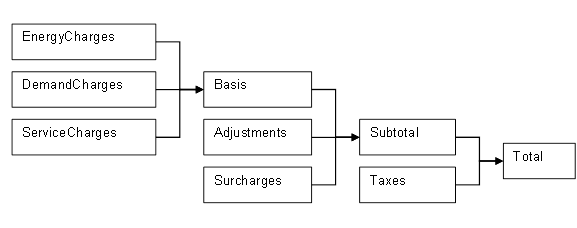
\includegraphics[width=0.9\textwidth, height=0.9\textheight, keepaspectratio=true]{media/image7909.png}
\caption{Category Hierarchy for Utility Bills \label{fig:category-hierarchy}}
\end{figure}

Any charges included in the EnergyCharges category are added together. The EnergyCharges, DemandCharges and ServiceCharges are added together to form the Basis. The Basis, Adjustments and Surcharges are added together to form the Subtotal. The Subtotal and Taxes are added together to be the Total.~ The total represents the total monthly charges on that tariff for the energy source used.~ The combining of categories together is performed automatically unless the user specifies the UtilityCost:Computation.~ In addition, each category, which is also a variable, may be used as a source. For example, a tax that is 5\% of the subtotal would be shown as:

\begin{lstlisting}

UtilityCost:Charge:Simple,
    TaxOfFivePercent,        ! Charge Variable Name
    TariffExample1,          ! Tariff Name
    Subtotal,                ! Source Variable
    Annual,                  ! Season
    Taxes,                   ! Category Variable Name
    0.05;                    ! Cost Per Unit Value (or Variable)
\end{lstlisting}

As you can see, the UtilityCost:Charge:Simple and UtilityCost:Charge:Block objects do most of the ``work'' of computing the annual energy cost.~ The benefit of using this categorization is that totals of each category are shown in the output reports and it organizes the charges in the monthly calculations in a logical way that fits almost all tariffs.~ If no categorization is desired, theoretically, all charges could be assigned to the Total category. The categories themselves are simply variable names. Charges may also be assigned to the ``NotIncluded'' category if the result of the charge is used as an intermediate calculation and should not be included in the Total.

The objects that create variables are:

\begin{itemize}
\item
  UtilityCost:Qualify
\item
  UtilityCost:Charge:Simple
\item
  UtilityCost:Charge:Block
\item
  UtilityCost:Ratchet
\item
  UtilityCost:Variable
\end{itemize}

\subsection{Default Order of Computation}\label{default-order-of-computation}

The user has the option of two different ways to determine the order of computation. If an UtilityCost:Computation object is specified for the tariff, the sequence specified in that object is used for computing the various variables. If no UtilityCost:Computation object is specified, a sequence of computational steps is automatically derived and shown as part of the report. The routine that creates this automatic sequence of computation steps is called CreateDefaultComputation as part of the EconomicTariff module.

The order in which the computation should be made is complicated by the fact that the objects can each have variables that are inputs and others that are outputs.~ Since any of the variables can be used as inputs, we must ensure that they are computed prior to being used. In other words, because the objects allow a great deal of flexibility, there is no simple default order that the computations should be made.

Luckily there are known algorithms for sorting though these types of interdependencies.~ In fact, the method that spreadsheets use for sorting through the dependencies of cell formulas referencing other cells with formula is very similar.~ In addition, linkers (used as part of the computer language compiling process) face similar issues of sorting through dependences. Figuring out the optimal path in a complex project represented by a PERT Chart also uses a similar algorithm.

Generically, dependency problems are usually characterized as Directed Acycle Graphs (DAGs). A DAG shows the individual formulas as circles and uses arrows between the circles to show which formula is dependent on which other formulas.~ One example algorithm that was used in EnergyPlus is described below:

\begin{itemize}
\item Calculate, for each node, the in-degree of that node (ie, now many edges end up there). Store these in array D.
\item Repeat:
\begin{itemize}
\item Remove (output) node such that D{[}n{]} = 0.
\item Decrement D{[}x{]} for all nodes x that are neighbors of n (edge from n to x).
\end{itemize}
\end{itemize}

Of course in this case ``node'' has nothing to do with EnergyPlus nodes but is just describing one of the formulas in a DAG.~ This is just one of several different methods to solve a DAG.~ The general method for solving a DAG is called a topological sort. The algorithm used in EnergyPlus is one of the simplest methods available and is appropriate given the number of dependencies.~ More efficient algorithms are known but are probably only appropriate for much larger number of dependencies.

One important note, if after the algorithm is exercised, and some of the formulas still have a count on the number of dependencies, it must be the result of a circular dependency and an error condition is flagged in the ERR file.

The objects have specific variables that are used as inputs and outputs, and thus the outputs are dependent on the inputs, are shown in Table~\ref{table:object-variables-input-output}.

\textbf{\emph{}}

\begin{longtable}[c]{@{}lll@{}}
\caption{Object Variables: Inputs and Outputs \label{table:object-variables-input-output}} \tabularnewline
\toprule 
Object & Outputs & Inputs \tabularnewline
\midrule
\endfirsthead

\toprule 
Object & Outputs & Inputs \tabularnewline
\midrule
\endhead

Qualify & Name & Source \tabularnewline
~ & ~ & Threshold \tabularnewline
Charge:Simple & Name & Source \tabularnewline
~ & Category & Cost Per Unit \tabularnewline
Charge:Block & Name & Source \tabularnewline
~ & Category & Block Size Multiplier \tabularnewline
~ & Remaining & Block Size \tabularnewline
~ & ~ & Block Cost \tabularnewline
Ratchet & Name & Baseline \tabularnewline
~ & ~ & Adjustment \tabularnewline
~ & ~ & Multiplier \tabularnewline
~ & ~ & Offset \tabularnewline
\bottomrule
\end{longtable}

In addition, the hierarchy shown in the first diagram in this section also represents dependencies that are included when determining the order of computation.

The resulting order of computation is shown at the bottom of the economics report.

\subsection{Computation Steps}\label{computation-steps}

Once the order that the formulas should be computed is known, the actual evaluation of the formulas is based on a simple Last In First Out (LIFO) stack.~ This is a common method to compute expressions where values are stored on the stack and operands work off of the top of the stack.
